\documentclass[12pt, oneside]{article}   	% use "amsart" instead of "article" for AMSLaTeX format
\usepackage[margin=1in]{geometry}                		% See geometry.pdf to learn the layout options. There are lots.
%\usepackage{cite}
\geometry{letterpaper}                   		% ... or a4paper or a5paper or ... 
\usepackage{graphicx}				% Use pdf, png, jpg, or eps§ with pdflatex; use eps in DVI mode
								% TeX will automatically convert eps --> pdf in pdflatex
\usepackage{titling}		
\usepackage{amssymb}
\usepackage{url}
\usepackage{titlesec}

\titleformat{\section}
  {\normalfont\fontsize{15}{15}\bfseries}{\thesection}{1em}{}
\titleformat{\subsection}  {\normalfont\fontsize{12}{15}\bfseries}{\thesubsection}{1em}{}

\setlength{\droptitle}{-5em}
%\setlength{\dropauthor}{-3em}

\pretitle{\begin{center} \Large}
\title{Predicting Chemical Fate Using Deep Learning: Progress Report}
\posttitle{\end{center} \lineskip 0.1em}
\preauthor{\begin{center} 
	\large \lineskip 0.1em}
\author{Zach Calhoun}
\postauthor{\par\end{center} \lineskip 0.5em}
\predate{\begin{center}\large}
\postdate{\par\end{center}}
%\date{}	

\begin{document}

\maketitle
%TODO - match formatting laid out in project description
\section{Project Objective}
For my final project, I want to explore how deep learning can be used to predict Henry's Law, a physical chemical property often used by environmental engineers to predict the fate of pollutants in the environment. Existing research has explored the ability of graph neural nets and variational auto-encoders to model chemical behavior well, but these have yet to be applied in the field of environmental chemistry, with most research seemingly in drug design and toxicology \cite{RN106}. Thus, my goal through this project is to learn about modeling chemicals using deep learning within the context of environmental chemistry, by building a model to predict Henry's law based on chemical structure.

\section{Problem Statement}
Roughly 10 million new chemicals are synthesized each year, and the EPA is only equipped to screen a fraction of these chemicals for environmental risk \cite{burton}. Of particular concern are so-called PBT (persistent, bioaccumulative, and toxic) chemicals. These chemicals are unique because they do not break down, they are particularly toxic, and because they bioaccumulate, they risk making their way into the food chain \cite{matthies}.

Perhaps the most infamous example of a PBT is DDT, the fertilizer used during the 20th century that was found to be highly toxic to bird populations, inspiring Rachel Carson's \emph{Silent Spring}. The more recent example making headlines today is PFAS (per-fluorinated alkyl substances), which represents the class of chemicals commonly found in non-stick pans or in water-repellant clothing. In both cases, the chemicals were synthesized for a particular purpose, and the risk to society was discovered decades later. Decades later, however, is far too late. Both PFAS and DDT are now ubiquitous, found in remote locations such as the Arctic, as well as in a large percentage of the population's bloodstream \cite{czub}.

To prevent this pattern from repeating itself, the EPA conducts environmental risk assessments using known and estimated chemical properties to predict chemical fate and toxicity in the environment. However, the EPA can only fully study a fraction of the compounds they need to, and estimations can be unreliable \cite{burton}. For example, the Bond Contribution Method is frequently used to predict Henry's law \cite{meylan}. This method is based on a small set of chemicals, and its output may be unreliable, since it only focuses on the bonds in the molecule rather than the structure as a whole. Deep learning, and specifically, Graph Neural Networks and Variational Auto-encoders both represent models that may be able to more effectively represent the impact of molecular structure on Henry's law.

If we could better predict this property, then environmental chemists could more accurately assess the true risk of new compounds on the market, allowing society to better prevent the widespread adoption of chemicals that pose significant environmental threats.

\section{Data Summary}
Henry's law (also called the air/water partitioning coefficient) is chosen because it is a well studied partitioning coefficient, meaning a lot of chemicals have values based on observations rather than estimations. For this project, I searched for a dataset that provided the Henry's law constant in a standardized format. That is, the values given for the constant need to have consistent units, be taken at standard temperature and pressure, and clearly indicate the source of the measurement, as it is vital that my model is trained on observed values, rather than calculated values. 

\subsection{Henry's Law Constants}
I found a compilation of Henry's law constants in \cite{sander2015}. This compilation contains over 17,000 values for over 4,600 chemicals. Each chemical had several values given, with sources including actual measurements, and a variety of estimation methods (e.g., a thermodynamical calculation was used to predict Henry's law). 

The author of this compilation provided the data through the webpage cited in \cite{sander-website}. Since the data was provided as a large SQL query, I ran the query using PostgreSQL to construct the tables needed to extract the data. I then selected all columns from  the \texttt{henry} table joined with the \texttt{species} table so that I could see a list of Henry's law values for each compound. This query was saved into a CSV file so that analysis could be done outside of SQL.

\subsection{Chemical Properties}
While the source mentioned above provided the Henry's law constants, this source did not provide the chemical properties needed to build a model. Most notably, many examples of predicting chemical properties from structure in machine learning make use of the Canonical SMILES (Simplified Molecular Input Line Entry System) representation of the chemical. The SMILES representation is a string representation of the chemical from which one can determine both the atoms comprising the molecule as well as the structure of the molecule, with the Canonical flavor of SMILES referencing the fact that each compound's SMILES representation is unique \cite{oboyle2012}.

To get this representation for each molecule, I used the package PubChemPy \cite{PubChemPy}. This open-source project is a package that accesses PubChem, an online search tool for obtaining chemical information, using PubChem's Power User Gateway \cite{kim2015}. This data source is assumed reliable since it is managed by the National Institute of Health, and the open source package is merely a convenient method for accessing this data.

Upon using PubChemPy, it was discovered that compound queries provided extra information that could be leveraged to predict Henry's law. For each compound, PubChem provides the complexity, molecular weight, TPSA, hydrogen bond acceptor count, hydrogen bond donor count, and a covalent unit count. While other information was provided, I only kept these features from each query as these values pertain to the chemical structure and physiochemical properties of the molecule, which should be useful for building my model.

\section{Preprocessing the data}
Given that there was one primary dataset, and an auxiliary dataset to fill in gaps, significant preprocessing was required to complete the dataset.

\subsection{Joining the Data}
First, the compilation of Henry's law constants was reduced to unique compounds with measured values. There were two values for two compounds, so the measurements were averaged to ensure one measured value per compound. Following this reduction, there were 1,025 compounds left over.

For each compound, PubChem was queried to get further information using the chemical's unique identifier (the Inchikey), which the compilation contained as a unique reference. For the 1,025 compounds, only those with 1 unique match in the PubChem database were kept. This resulted in a dataset containing 960 compounds, which was the final dataset used in my analysis.

\subsection{Log Transform}
Values for Henry's law fall in the range of 0 to infinity. If the value is zero, the compound may vaporize almost immediately out of its aqueous phase into the atmosphere, and an infinite value indicates that the compound strongly prefers the aqueous phase. I use the term infinite here to indicate the theoretical limit, but in practice, a strongly hydrophilic, or water-loving, compound will have a very large constant. In this dataset, the range of observed values is $(1.2\times10^{-7}, 2.3\times 10^{10})$. % TODO - insert here.

To address this large difference, I performed a log-transform on the Henry's law values, to get the distribution shown in Figure~\ref{fig:dist}. This additionally makes sense from a practical point of view; environmental engineers often care about the order of magnitude rather than the actual value when calculating Henry's law.

\begin{figure}[h!] %  figure placement: here, top, bottom, or page
   \centering
   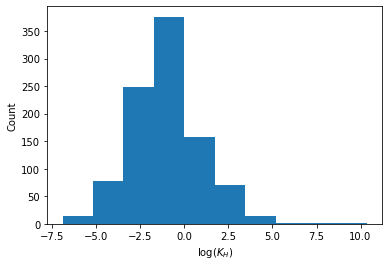
\includegraphics[width=4in]{data-dist.png} 
   \caption{The Distribution of $\log K_H$, where $K_H$ refers to the Henry's Law Constant.}
   \label{fig:dist}
\end{figure}


\section{Methods and Results}
The dataset was compared to the estimated values where they existed in the Henry's law compilation to get a baseline mean squared error (MSE) of 0.2-0.8, depending on the method. However, both measured and estimates only existed for a small subset of the data.

An initial model was built using just the physical properties provided by PubChem. For this initial attempt, the data was split into an 80/20 train/test set. I initially wanted my model to be interpretable, so I tried a simple decision tree regressor model. With a max depth of 6, this model had an MSE of $1.5$. I then built a Random Forest Regressor, which decreased the MSE to $1.4$. This performance was mostly invariable to changing hyper-parameters, so this set a base line for my models.

Next, I wanted to see how well a model could perform just using the structure. To do this, I converted each chemical to its embedding using the Mol2Vec pre-trained embeddings, as referenced in \cite{jaeger2018}. The embeddings are a 300 dimensional representation of each substructure within a molecule. For each compound, the substructures were summed to get one 300 dimensional vector for each compound. I then created a KNeighborsRegressor, with the optimal number of neighbors equal to 8 to get a test set MSE of $1.4$. 

Because 300 dimensions is likely too many dimensions for a dataset of 960 examples, I then ran Principal Component Analysis to attempt to reduce the dimensionality. About 5 principal components explained 80\% of the variance, so K Nearest Neighbors was attempted on this reduced dimensionality dataset. This time, an optimal MSE of $1.5$ was found with 10 neighbors.

My initial results seems promising, but I believe the information from the molecule substructures might be better aggregated (as opposed to summing the molecule vectors), and by exploring methods for dimensionality reduction.

\section{Conclusions}
I have created models using physical chemical properties, and models only using the structure, and these models perform very similarly. Given that my initial goal was to learn how to predict environmentally relevant chemical properties using only structure, my initial results suggest that this approach can be applied with success.

My next steps will be to determine whether alternative methods could improve performance. I suspect that my dataset size is preventing performance from increasing, so my focus will be on dimensionality reduction techniques and refined application of the embeddings provided by the Mol2Vec package. Previous research has demonstrated the efficacy of Variational Auto-Encoders applied to chemical footprints to enhance prediction of chemical toxicology \cite{RN106}. I believe a similar approach may be useful in this domain.

After applying this final approach, I will assimilate my approaches and compare them to the estimation approaches to further explore how my models are performing. I have created several models already, so further analysis is required to evaluate these models to understand the results so that my final report will contain more thorough analysis to better understand this problem space.

\bibliography{ds4cee-final-project}{}
\bibliographystyle{ieeetr}

\end{document}  